\documentclass[amsmath,amssymb, aps, prl, twocolumn]{revtex4-1}

\usepackage{graphicx}% Include figure files
\usepackage{dcolumn}% Align table columns on decimal point
\usepackage{bm}
\usepackage[usenames]{color}

\begin{document}

%\title{Machine learning transport with quantum loop topography}
\title{ Probing transport in quantum many-fermion simulations\\ via quantum loop topography}

\author{Yi Zhang$^1$}
\email{frankzhangyi@gmail.com}
\author{Carsten Bauer$^2$}
\author{Peter Broecker$^2$} 
\author{Simon Trebst$^2$}
\author{Eun-Ah Kim$^1$}
\email{eun-ah.kim@cornell.edu}

\affiliation{%
$^{1}$Department of Physics, Cornell University, Ithaca, New York 14853, USA}%
\affiliation{$^{2}$Institute for Theoretical Physics, University of Cologne, 50937 Cologne, Germany}

\date{\today}% It is always \today, today,
             %  but any date may be explicitly specified

\begin{abstract}
Quantum many-fermion systems give rise to diverse states of matter that often reveal themselves in distinctive transport properties. While some of these systems can be captured by microscopic models accessible to numerical exact quantum Monte Carlo simulations, it nevertheless remains challenging to  numerically access their transport properties. 
Here we demonstrate that quantum loop topography (QLT) can be used to directly probe transport by machine learning current-current correlations in imaginary time.
We showcase this approach by studying the emergence of superconducting fluctuations in the negative-U Hubbard model and an effective action model for an antiferromagnetic quantum critical point. For both models
we find that the QLT approach detects a change in transport in very good agreement with their established phase diagrams.
%derived from conventional numerical estimators.
These proof-of-principle calculations combined with the numerical efficiency of the QLT approach point a way to identify elusive
transport phenomena such as non-Fermi liquids using machine learning
algorithms.

%One of the major challenges in condensed matter physics is to process the `big data', being it the Hilbert space of the quantum many-body states or the data generated from modern-day experiments and large-scale computations. Recently, machine learning techniques have been introduced into condensed matter physics research and exhibit great strengths in applications handling such `big data'. Here we show that via supervised machine learning, artificial neural networks can successfully identify the emergent superconductivity with different pairing symmetries and from various interacting fermion models. In particular, we focus on the mere samples of the two-point correlations, which are readily available in Determinant Quantum Monte Carlo calculations and avoid the conventional yet complex procedures for the superfluid density. Instead, we show that with either a quantum loop topography feature-selection layer or deep convolutional layers, the empowered neural networks achieve trustworthy performance based upon the raw data of correlations, therefore greatly reduce the computational cost.
\end{abstract}

\maketitle

\section{Introduction}

Key challenge with studying quantum many-fermion systems has to do with the fact that the defining macroscopic characteristic of a state is often its transport property. Unfortunately, 
rigorous information on transport one can gain from Monte Carlo simulations is limited because Monte Carlo simulations yield imaginary time data, and the analytic continuation of imaginary time data to real time is numerically ill posed. Nevertheless, the imaginary time current-current correlation function must contain the nugget of the key information regarding transport. Indeed 
superfluid density can be rigorously obtained to signal superconductivity\cite{Scalapino1993} and even a “proxy” for the DC resistivity can be obtained to hint at non-Fermi liquid behavior\cite{Lederer2017}, all starting from current-current correlation function. Therefore it is plausible that a machine learning approach that targets information relevant for current-current correlation can enable efficient acquisition of phase diagrams by probing qualitative change in transport.

{\color{red} (Simon: We need to go from many-fermion to QMC. We may not want to bring in quantum criticality.)} Quantum criticality with itinerant fermions can be studied exactly in sign-problem free models that are nevertheless quite rich \cite{Berg2012,Schattner2016a,Gerlach2017,Xu2017a,Lederer2017,Li2016,Li2017,Jiang2017}, motivating interest in studying phase diagrams of variety of  “sign-free” models. Nevertheless, ``sign-free'' does not imply ready accessible. 
In fact, scanning the multi-dimensional phase space can be quite time-consuming, even if the absence of the sign problem makes the cooling down to low-temperatures possible in principle. One approach to speeding-up Monte Carlo simulations using machine learning is to making each update more efficient by either increasing the acceptance rate using the restricted Boltzmann machines to propose updates\cite{Huang2017}, or finding an approximate Hamiltonian to guide update suggestions\cite{Liu2017}. 
An alternative is to minimize the number of necessary updates by using the ANN’s ability to “see through” a noisy data. {\color{red} (Simon: a summary of literature here ending with importance of input?)}



In this paper, we adapt the QLT first introduced in Ref.~\cite{qlt2016} for the topological Hall response to the longitudinal transport.  {\color{red}(EK: a few words on how QLT worked for topological response.)}
%Machine learning techniques have emerged as an effective alternative to big data analysis and regression towards the underlying clues in abstract entities such as images and voices\cite{MLbook}. Recently, machine learning have shown exciting developments in the territories of the condensed matter physics, where similar 'big data' issues have laid increasing challenges in researches. Indeed, methods such as the neural network states\cite{Carleo2016, Deng2016, Deng2017, Glasser2018, Torlai2018, Gaoxun2017} and self-learning simulations\cite{Meng2016, Leiwang2017, Junwei2017b, Junwei2017c} have largely impacted our capacity towards representing quantum many-body states. On the other hand, it is vital to identify the corresponding phases of the many-body states, which characterize the low-energy collective behaviors and dominate their general properties. It is the similarity between this task and the iconic success of machine learning in image recognition that has inspired the rapid progress of applying machine learning techniques to phase recognition\cite{Melko20161, Nieuwenburg2017, LeiWang2016, Simon2016, Kelvin2016, Ohtsuki2016, Ohtsuki2017, Titus2017, qlt2016, FrankMLZ2, Broecker2017, ZhaiHui2017, Iakovlev2018, PollmannML2018, Anna2018}, especially for difficult problems involving strong correlations and topological phases that defies conventional approaches. 
%Superconductivity is the fascinating phenomena of exactly zero electrical resistance and expulsion of magnetic fields. Despite the vast diversity among the conventional phonon-assisted BCS superconductors and the unconventional superconductors such as the Cu-based, Fe-based and heavy-Fermion materials, they are universally characterized by electrons forming Cooper pairs. On the other hand, unlike other Landau symmetry breaking phases, the superconductors break the $U(1)$ gauge symmetry. Except for the mean-field theories that explicitly break the charge conservation, a well-defined order parameter signaling the symmetry breaking is not immediately available for emergent superconductivity. Pair correlation offers a partial substitute yet still decays in two dimensions making identification ambiguous in finite size systems. A more established signature is the advent of a non-zero superfluid density $\rho_s$, obtainable from the longitudinal and transverse current-current correlations\cite{Superfluids, Scalapino1992, Scalapino1993, Nandini1996}. For this purpose, we need to measure the current-current correlations $\Lambda_{xx}$ across the entire real space as well as the imaginary time. This requires a large number of samples in a Monte Carlo simulation in order to suppress the uncertainty, especially for correlations over distances with small expectation values. Then, we Fourier transform, extrapolate to the long-wavelength limits $\omega=0, q_x\rightarrow0, q_y=0$ and $\omega=0, q_x=0, q_y\rightarrow0$, and take the difference. The overall cost for a clear-cut detection of the superconductivity is still rather high, especially near the superconducting transition where the value of $\rho_s$ is small.
%In this paper,  we use supervised machine learning for purpose of detecting emergent superconductivity from interacting fermionic systems.
Here we consider emergent $s$-wave superconductivity in the negative $U$ Hubbard model\cite{Scalettar1989, Scalapino1992} and the emergent $d$-wave superconductivity in models where the Fermi surfaces are coupled to a $\vec Q=(\pi, \pi)$ spin density wave (SDW) order parameter\cite{Erez2016}. Both models can be simulated via Determinant Quantum Monte Carlo (DQMC) methods without the sign problem. %Instead of calculating the superfluid density, we focus on the two-point correlations as our raw data source, which are conveniently available in DQMC calculations. Two artificial neural network (ANN) architectures are applied in parallel: a deep neural network with convolutional layers\cite{Simon2016}, and a shallow neural network with a feature selection layer dubbed as quantum loop topography\cite{qlt2016, FrankMLZ2}, focusing on correlations trailing three-point and four-point loops at the shortest length scales. Both architectures have their respective merits: while the deep convolutional neural network is powerful enough to minimize our human intervention, the introduction of quantum loop topography as humanly inspired by the physical relevance of the information - the current-current correlations in this case - helps to reduce the complexity of the ANN and the corresponding efforts for supervised machine learning. We train our artificial neural networks with data deep in the superconducting phases at low temperature and normal phase at high temperature. Benchmarks suggest that in both scenarios we can achieve good performance with a small number of uncorrelated Monte Carlo samples, therefore largely reduce the computational cost of the conventional algorithm. 
%Although our examples are two-dimensional models, it is straightforward to generalize the methods to other dimensions. 

\section{quantum loop topography for longitudinal transport}
The Quantum loop topography (QLT) is a preprocessing step for machine learning quantum many-body models~\cite{qlt2016} that selects and organizes the simulation data with the physical response characteristic of the target phase in mind. Targeting the longitudinal transport,  we built a vector at each site $j$ consisting of all small loops with three vertices, $L^\triangle_{jkl}$ and with four vertices, $L^\Box_{jklm}$ including the site $j$. The loops represent
chained products of bi-linear operators  $c_i^\dagger c_j$ evaluated with a single Monte Carlo sample $\alpha$, $\widetilde{P}_{jk}|_{\alpha}$:
\begin{equation}
    L^\triangle_{jkl}\equiv\widetilde{P}_{jk}|_{\alpha} \widetilde{P}_{kl}|_{\beta} \widetilde{P}_{lj}|_{\gamma},
    \label{eq:triangle}
\end{equation}
and 
%limiting the neighboring sites to be within a short-distance cutoff $d_c$. 
%Now in order to target the longitudinal transport, in addition to the triangular loops %$L^\triangle_{jkl}$ in Eq.~\ref{eq:triangle}, we use quadralateral loops $L^\Box_{jklm}$:
\begin{equation}
L^\Box_{jklm}\equiv\widetilde{P}_{jk}|_{\alpha'} \widetilde{P}_{kl}|_{\beta'} \widetilde{P}_{lm}|_{\gamma'} \widetilde{P}_{mj}|_{\delta'},
\label{eq:quad}
\end{equation}
limiting the neighboring sites to be within a short-distance cutoff $d_c$. See Fig.~\ref{fig:loops} for the loop operators associated with site $1$ with the shortest lengths.

\begin{figure}
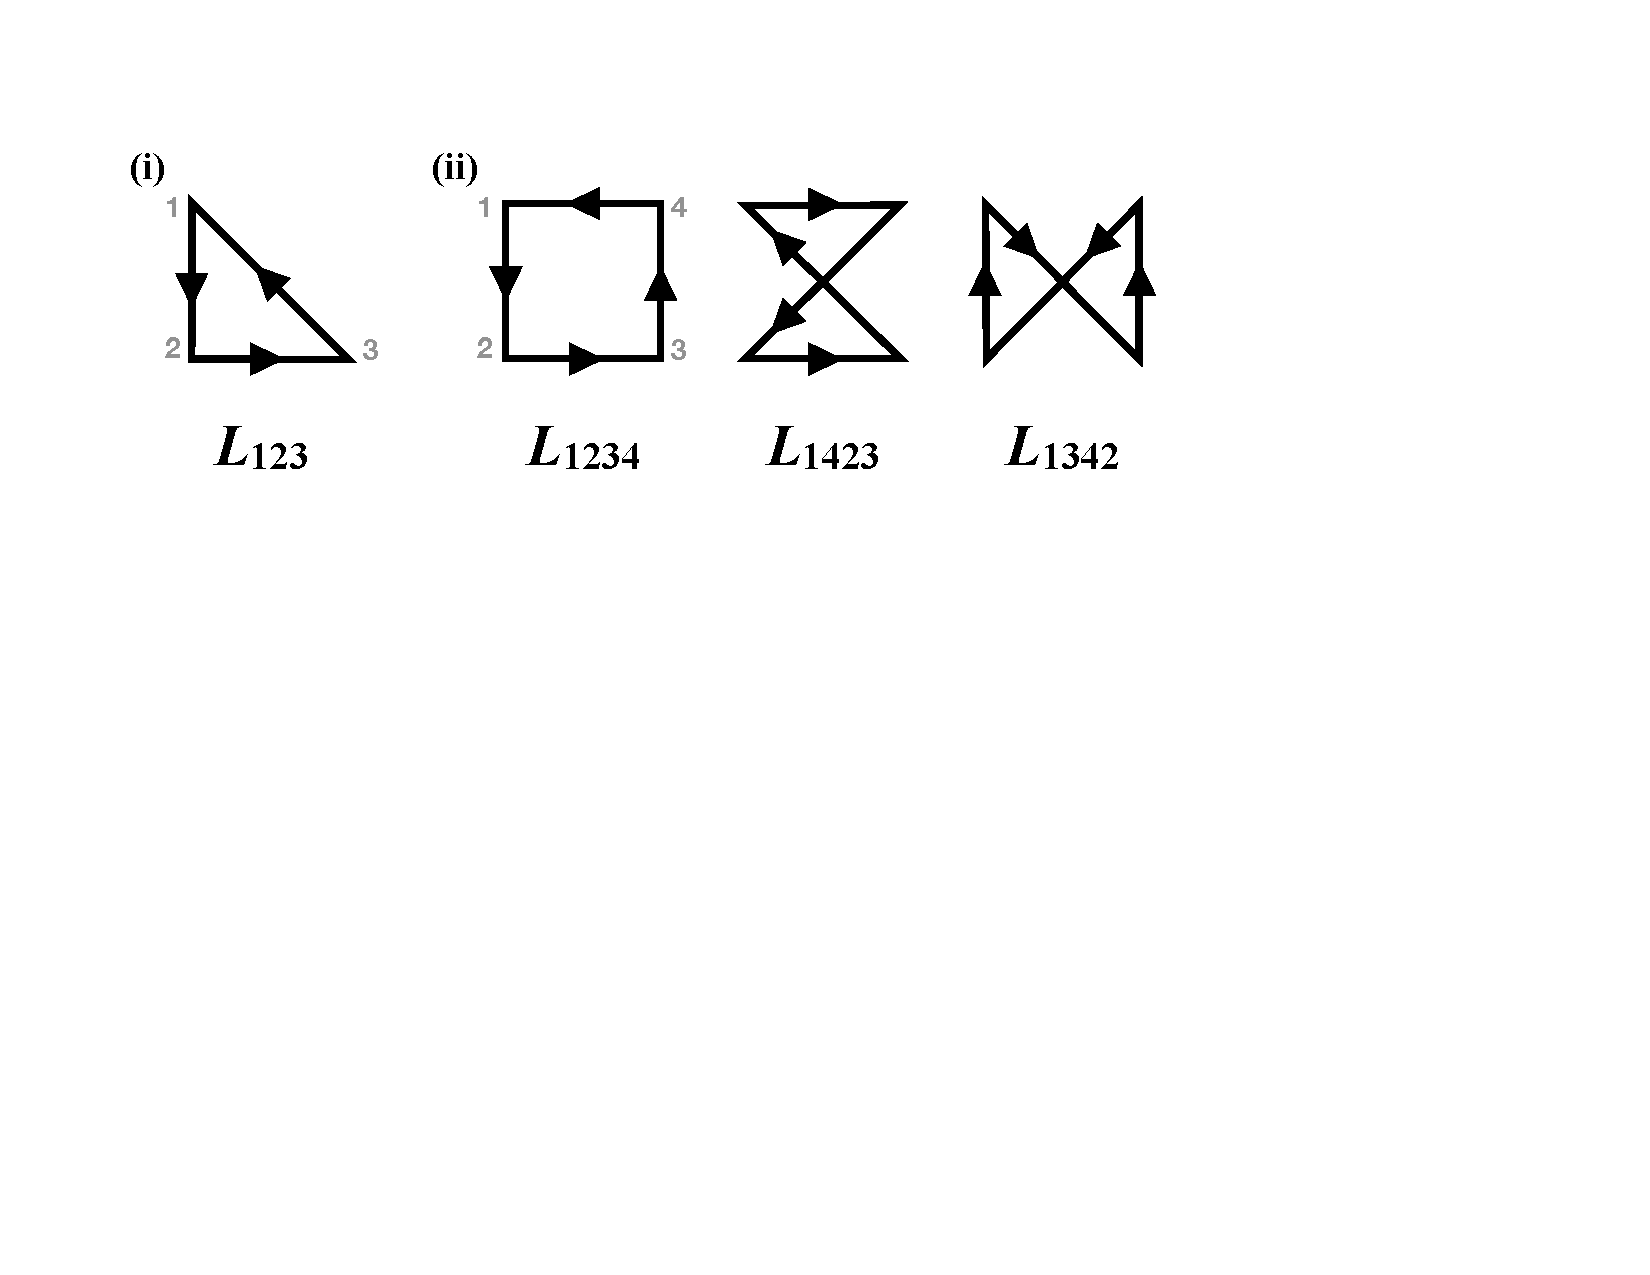
\includegraphics[scale=0.48]{LoopOperators.pdf}
\caption{
 Illustration of the (i) triangular and (ii) quadralateral {\bf loop operators} employed to calculate the longitudinal transport. 
}\label{fig:loops}
\end{figure}

To see how the loop operators $L^\Box_{jklm}$ and $ L^\triangle_{jkl}$ capture the longitudinal transport, consider the zero-frequency current-current correlation function:  
\begin{equation}
\Lambda_{xx}({\bf r}_1,{\bf r}_2;\omega_n=0)\equiv\int d\tau\left\langle j_x\left({\bf r}_1, \tau \right) j_x\left({\bf r}_2, 0 \right)\right\rangle,
\label{eq:Lambda}
\end{equation}
where $j_x({\bf r}_1,\tau)=e^{H\tau} j_x({\bf r}_1) e^{-H\tau}$ with 
$j_x({\bf r_1})= [H,{\bf r}_1]$ {\color{blue}(Frank: check)}. The Fourier transform of the 
current-current correlation function in Eq.~\eqref{eq:Lambda} is famously related to the superfluid density $\rho_s$ through $\rho_s=\Lambda_{xx}(q_x\rightarrow 0,\omega_n=0)-\Lambda_{xx}(q_x=0,\omega_n=0)$ {\color{blue}(Frank: check)}. 

%$\left|G\right\rangle$ is the target ground state. 
%Given the imaginary time evolution $j_x(r_1,\tau)=e^{H\tau} j_x(r_1) e^{-H\tau}$,
%\begin{eqnarray}
%& &\int d\tau \left\langle j_x\left(r_1, \tau\right) j_x\left(r_2, 0 \right)\right\rangle
%\nonumber\\
%&=&\sum_{n\ne G} \frac{\left\langle G \left| j_x(r_1)  \left|n\left\rangle  \right\langle n\right| j_x(r_2)\right| G\right\rangle}{E_n-E_G}.
%\label{eq:lambdaform}
%\end{eqnarray}
Now a rigorous relationship between the Loop operators $L^\Box_{jklm}$ and $ L^\triangle_{jkl}$  and 
the longitudinal current response can be established for a gapped spectrum at zero temperature. {\color{blue}For a gapped hamiltonian, the Hamiltonian can be approximated by a flat band Hamiltonian  $H'=-\hat{P}$ (Frank: we still need to update this to be related to MF BdG)} with the 
%if we consider
the projection operator
$\hat{P}\equiv |G\rangle \langle G|$ where $|G\rangle$ is the ground state. Now for the system with the Hamiltonian $H'$ at zero temperature %, the right hand side of Eq.~\ref{eq:lambdaform} simplifies to 
%and approximate the Hamiltonian $H'=-P$. $H'$ is adiabatically connected to $H$ in the gapped phase yet it has a simpler flat excitation spectrum $E_n-E_G=1$. Now 
\begin{eqnarray}
    %\sum_{n\ne G} \frac{\left\langle G \left| j_x(r_1)  \left|n\left\rangle  \right\langle n\right| j_x(r_2)\right| G\right\rangle}{E_n-E_G}
   \Lambda_{xx}({\bf r}_1,{\bf r}_2;\omega_n\!=\!0) &=& \langle G|j_x({\bf r}_1)(1-\hat{P}) j_x({\bf r}_2)|G\rangle \nonumber\\
   &=&{\rm Tr}\ \hat{P}j_x({\bf r}_1)(1-\hat{P}) j_x({\bf r}_2),
\end{eqnarray}
where we set the gap energy scale to be 1.
%where we have suppressed the position arguments. 
For a mean-field Bogoliubov deGenne hamiltonian with flat band, the trace can be evaluated to be (see Appendix for further detail)
%urther using the fact that current density is given by the commutator of the Hamiltonian and the position operator, we obtain
\begin{eqnarray}
%P j_x \left(1-P\right) j_x &=& - P \left[H',x\right] \left(1-P\right) \left[H',x\right] \nonumber\\
\Lambda_{xx}({\bf r}_1,{\bf r}_2;\omega_n\!=\!0)&=& P_{ij}P_{jk}P_{kl}P_{li} \left(x_j-x_k\right)\left(x_l-x_i\right) \nonumber\\&-& P_{jk}P_{kl}P_{lj}\left(x_k-x_l\right)\left(x_l-x_j\right)
\label{eq:j-j}
\end{eqnarray}
where we have suppressed the position-space indices in the first line and implied the summations over the subscripts and trace over the spins in the last two lines. {\color{blue}(Frank: fill in the indicies that are not being summed over to make r1 and r2 explicit.)}

Hence for the approximate hamiltonian $H'$, the current-current correlation function consists of appropriately weighed combination of quadrilateral loops and triangular loops of all sizes.
Since NN's can learn to form the relevant combination of the inputs we use both $L^\triangle_{jkl}$ and  $L^\Box_{ijkl}$ defined in Eqs.~\ref{eq:triangle} and \ref{eq:quad} as inputs. 

Note that we use Determinent quantum Monte Carlo (DQMC) samples of the Green's functions $\widetilde{P}_{jk}|_{\alpha}$. Such data is intrinsically fluctuation-laden, yet it allows us to generate abundant samples for a given model, and at the same time reduces the computation cost and necessary Monte Carlo steps for the phase identification\cite{qlt2016, FrankMLZ2, Simon2016, Kelvin2016}. After the ANN is trained and optimized with samples from low and high temperatures with the pre-existing labels, the resulting ANN is used to identify the superconducting transport at intermediate temperatures based upon their respective DQMC samples.  

We feed the samples of the quantum loops $L^\Box$ and $ L^\triangle$ as our `images' into a feed-forward fully-connected shallow neural network with only one hidden layer consisting of $n=40$ sigmoid neurons for both training and testing purposes. Each neuron processes the input $x$ through independent weights and biases $w\cdot x+b$. After the sigmoid function, the outcome is fed forward to be processed by the output sigmoid neuron. The final output $y$ corresponds to the neural network's judgment whether the input source is superconducting ($y>0.5$) or not ($y<0.5$).
For supervised machine learning, we use cross-entropy cost function, L2 regularization to avoid over-training and a mini-batch size of 10. We also reserve an independent validation set $10\sim 20\%$ of the size of the training set for validation purposes including learning speed control and termination\cite{MLbook}.

Clearly, the loop operators $L^\Box_{jklm}$ and $ L^\triangle_{jkl}$ as defined in \eqref{eq:triangle} and \eqref{eq:quad} built from single Monte Carlo instances only for short-ranged loops, cannot replace a rigorous calculation of current-current correlation function, especially for a gaples system. But we anticipate the QLT consisting of the triangular and quadrilateral loops serve as a proxy for the current-current correlation function containing qualitative information regarding longitudinal transport directly in the imaginary time data.  

%Since NN's can learn to form the effective combination of the inputs, Eq.~\ref{eq:j-j} suggests that use of both $L^\triangle_{jkl}$ and  $L^\Box_{ijkl}$ defined in Eqs.~\ref{eq:triangle} and \ref{eq:quad} as inputs could enable ANN's to probe transport properties in imaginary time data. Throughout the rest of this paper we focus on only the loops with the smallest length scales, since the correlation $P$ decays over distances. For the rest of the paper, we only include the quantum loops $L$ and $L'$ whose width is equal or below a cut-off scale $d_c=2$ unless noted otherwise.





\section{Models and Results}
To test the potential of the QLT for efficiently detecting qualitative difference in the transport from imaginary time Greens function data, we consider models that host superconductivity in parts of the phase space. {\color{blue}A rigorous detection of the onset of superconductivity requires XXX within DQMC since the superconducting order parameter itself is not directly accessible in DQMC which conserves particle number by construction. One can also do YYY to detect the existence of superconducting fluctuation.}

We first consider the negative $U$ Hubbard models on a two-dimensional square lattice\cite{Scalettar1989, Scalapino1992} which is a well-studied model that can serve as a benchmark. 
\begin{eqnarray}
H &=& H_0 + H_U -  \mu\underset{i}{\sum} \left(n_{i,\uparrow} +n_{i,\downarrow}\right) \nonumber\\
H_0 &=& -\underset{\left\langle ij \right\rangle, s}{\sum} \left( c^\dagger_{j,s}c_{i,s} +  c^\dagger_{i,s}c_{j,s} \right) \nonumber \\
H_U &=& U \underset{i}{\sum} \left(n_{i,\uparrow}-\frac{1}{2}\right) \left(n_{i,\downarrow}-\frac{1}{2}\right)
\label{eq:hubbard}
\end{eqnarray}
where $s = \uparrow, \downarrow$ denotes the spin, $c^\dagger_{i,s}$ is the electron creation operator, and $n_{i,s}=c^\dagger_{i,s}c_{i,s}$ is the electron density operator. $U=-\left|U\right|<0$ is the attractive interaction strength and $\mu$ is the chemical potential. Without loss of generality, we set $U=-8$ and the chemical potential $\mu=XX$ slightly below neutrality, corresponding to an average electron density $\left\langle n\right\rangle = \left\langle n_\uparrow\right\rangle+ \left\langle n_\downarrow\right\rangle  \simeq 0.9$ slightly below half filling. We set the system size to $8\times 8$. 


%After proper Trotter decomposition and mapping the system into 2+1 dimensions with the imaginary time direction controlling the systematic temperature, both models can be simulated via DQMC methods without the sign problem. Both models exhibit a superconductor-metal transition at a critical temperature\cite{Scalettar1989, Scalapino1992,Erez2016}. On the other hand, while the pairing symmetry is naturally $s$-wave in the negative $U$ Hubbard model, the low-temperature superconducting phase of the effective action model in Eq. \ref{eq:afmetal} that consists two flavors of fermions coupled to an SDW order parameter and exhibits $d$-wave pairings. 

\begin{figure}
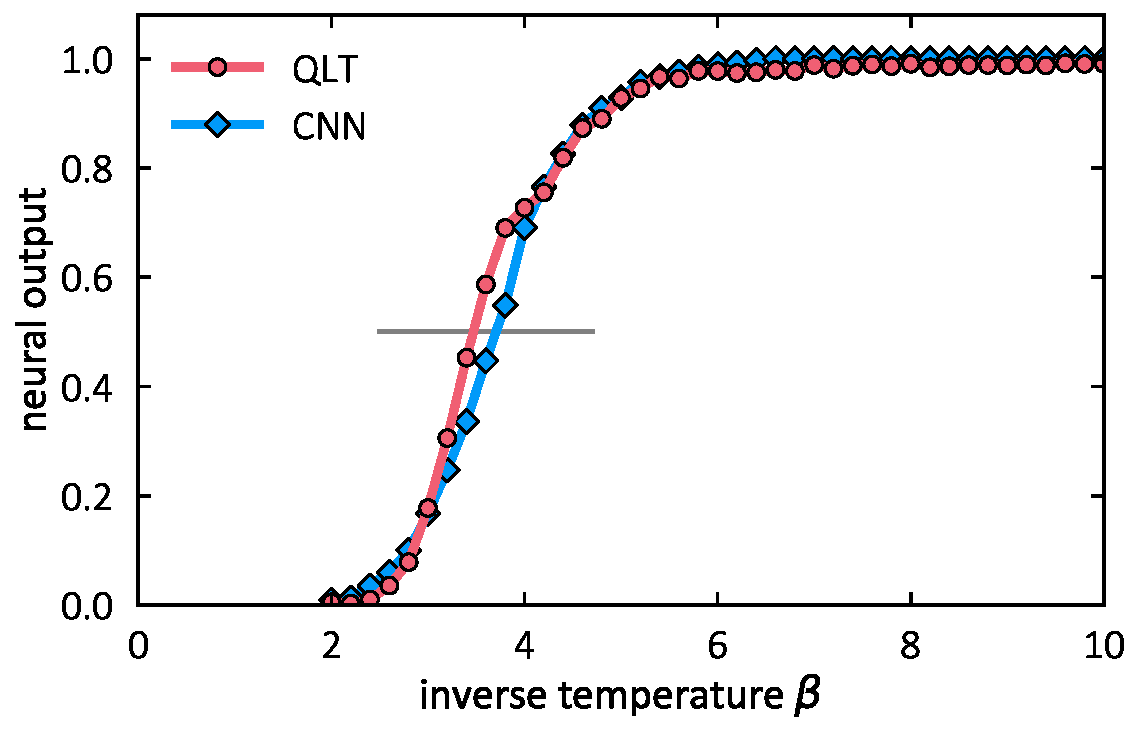
\includegraphics[scale=.43]{fig1.pdf}
\caption{
{\bf Negative-U Hubbard model.} The neural outputs of the quantum loop topography (QLT) and convolutional neural network (CNN) architectures for superconducting transport versus the inverse temperature $\beta$. While the inputs for the deep CNN are the unprocessed Green's functions $P(r,r')$ from the square-lattice negative $U$ Hubbard model in Eq. \ref{eq:hubbard}, we pre-process the input for the shallow ANN of the QLT architecture in the form of the quantum loops in Eq. \ref{eq:triangle} and \ref{eq:quad}. Both architectures are trained with samples at low temperature $\beta=20$ representing superconducting transport and high temperature $\beta=2$ representing normal state transport. Then the resulting architectures are applied towards the interpolating temperatures. $U=-8$, $\left\langle n\right\rangle= \left\langle n_\uparrow\right\rangle+\left\langle n_\downarrow\right\rangle\simeq 0.9$, $d_c=2$, and the system size is $8\times 8$. }\label{fig:hubbard}
\end{figure}

%Our neural network can successfully distinguish the superconductors from the normal metals irrespective of the superconducting pairing symmetry. First, this is illustrated using DQMC samples of the negative $U$ Hubbard model in Eq.\ref{eq:hubbard}. 
The training set consists of about 20,000 samples obtained from the superconducting phase at low temperature $\beta=20$ and normal metallic phase at high temperature $\beta=2$. %We perform two parallel studies using the both the CNN and the QLT architectures that we have proposed in the previous section. 
The results of the supervised machine learning on the interpolating $\beta$ are summarized in Fig. \ref{fig:hubbard}. %The results from the CNN are in very good consistency with the results from a simple neural network accompanying QLT, and both 
show very high accuracy and confidence $>99\%$ in the low temperature and high temperature limits. On the other hand, both neural network architectures suggest a transition near $T_c =\beta^{-1} \sim 0.28$; in comparison, superfluid density $\rho_s$ measurement suggested critical temperature $T_c\simeq 0.1$ for the superconductor-metal transition\cite{Scalapino1993}. %We note the thermal transition from a two-dimensional superconducting phase to a normal metallic phase is characterized by the Kosterlitz-Thouless transition type and the deconfinement of topological vortexes. The superconducting temperature is determined by $\rho_s(T_c)/T_c=2/\pi$ with a finite superconducting density $\rho_s$ at $T_c$, suggesting that the onsets of superconducting fluctuations and transport behaviors happen above the critical temperature. 
\begin{figure}
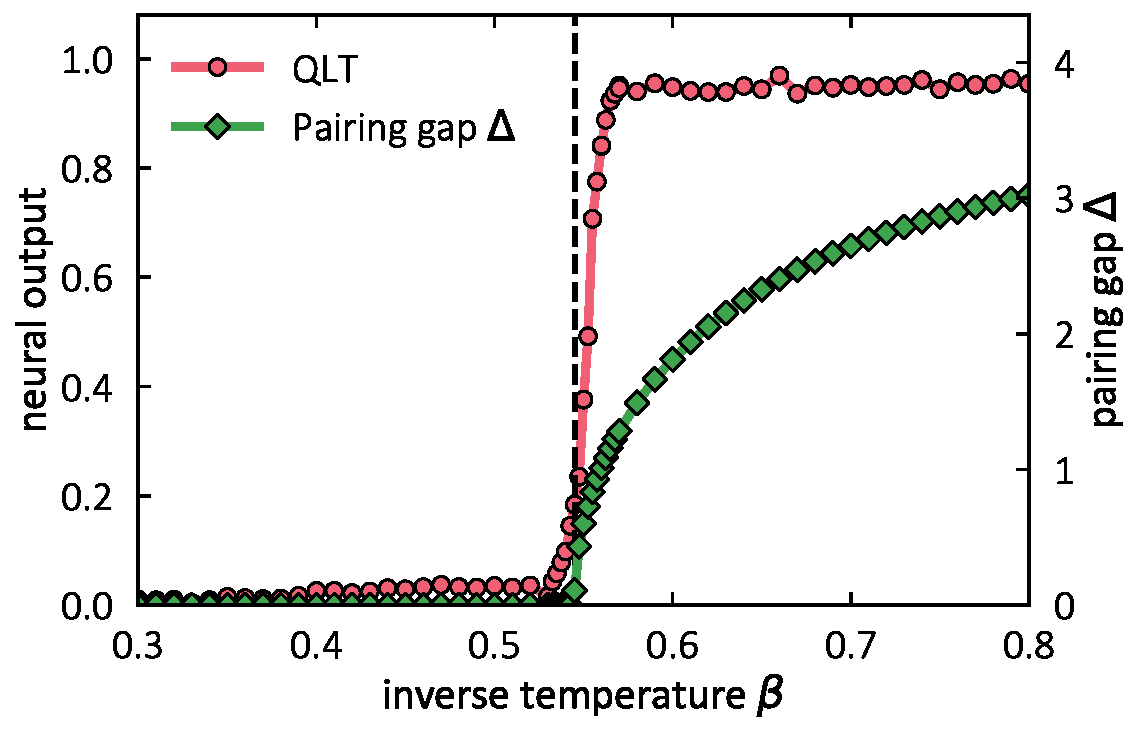
\includegraphics[scale=.43]{fig2.pdf}
\caption{{\bf Mean field theory of the Negative-U Hubbard model.} The mean-field $s$-wave pairing gap $\Delta$ follows the self-consistent gap equation at an inverse temperature $\beta$. The neural output from the QLT architecture is consistent with the debut of the superconducting gap. Here, we obtain the samples of the Green's function $P(r, r')$ through finite-temperature Monte Carlo calculations. $U=-8$, $\mu=-0.5$. The transition temperature $\beta_c\sim 0.545$ is shown as the vertical dashed line. A higher resolution is imposed near $\beta_c$ for clarity.}\label{fig:mlmft}
\end{figure}


 The other architecture we consider is a state-of-the-art deep convolutional neural network (CNN). Such CNN has succeeded in identifying phases and locating phase transitions in quantum many-fermion systems based on raw samples of the Green's functions\cite{Simon2016} without preprocessing. % The neural network consists of two sets of convolutional and max pooling layers followed by two fully-connected layers separated by a dropout layer. The neurons in the final layer has a softmax activation function, while all other neurons are set to be rectified linear units.

%This observation is also consistent with the performance of the neural network on mean-field ansatz, where the superconducting transport onset as soon as a mean-field pairing gap opens. For instance, 
We consider the mean field theory of the negative $U$ Hubbard models in Eq. \ref{eq:hubbard}, and determine the $s$-wave pairing gap $\Delta(\beta)$ at each inverse temperature $\beta$ through the self-consistent gap equation. In the corresponding BdG mean-field model with the respective $\Delta(\beta)$, we sample the quasi-particle occupation and generate samples of the Green's function $P(r,r')$ through finite-temperature Monte Carlo calculations. Then, a neural network with inputs processed through QLT is trained at  high ($\beta=0.3$) and low ($\beta=0.8$) temperatures and applied towards the intermediate temperatures. The results for $U=-8$ and $\mu=-0.5$ are shown in Fig. \ref{fig:mlmft}. We find a sharp transition that clearly aligns with the superconducting transition temperature. Note that our neural network can obtain an accurate decision with $\sim O(10)$ uncorrelated Monte Carlo steps\footnote{This includes the steps needed in constructing the quantum loops as well as the multiple tests to streamline the accuracy.}, a huge reduction over the required samples necessary for suppressing uncertainties in the superfluid density measurements\cite{Hong2016, Erez2016}. 

\begin{figure}
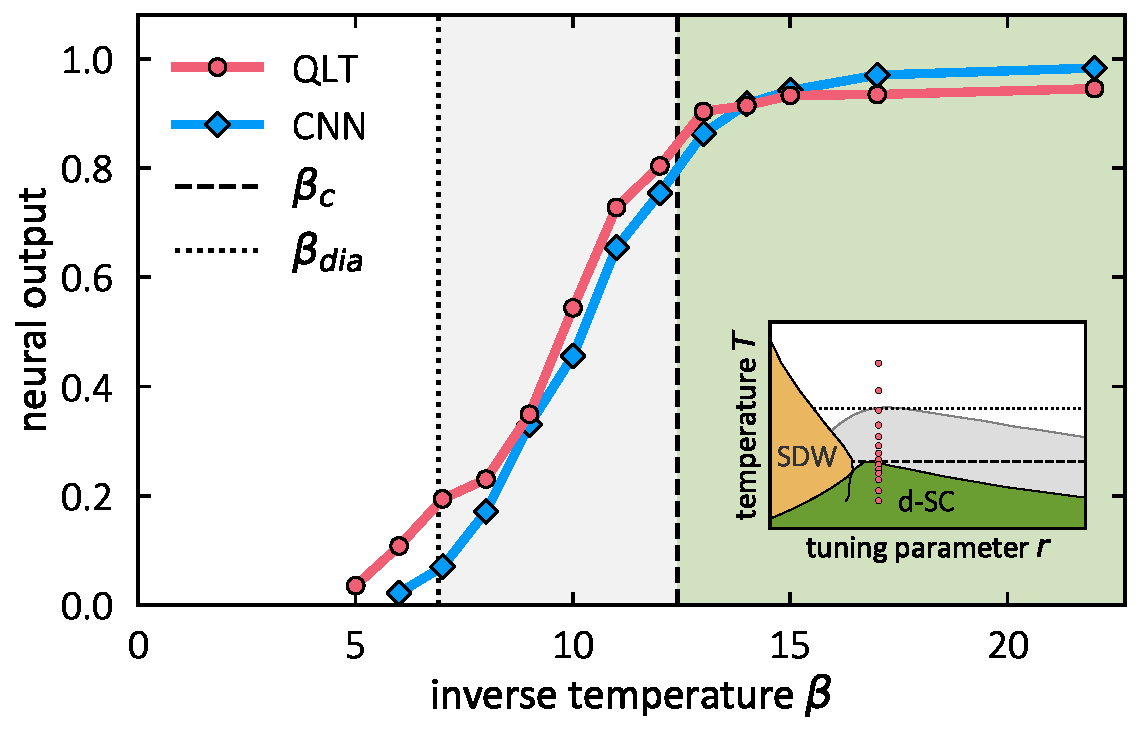
\includegraphics[scale=.43]{fig3.pdf}
\caption{{\bf Effective action model.}}
\label{fig:afmetal}
\end{figure}

 The second example we consider is a spin-fermion model in which two flavors of spin$-1/2$ fermions $\psi_x$ and $\psi_y$ are coupled to an easy-plane SDW order parameter $\vec{\varphi}$ at wave vector $\vec Q=(\pi, \pi)$ on a two-dimensional square lattice\cite{Erez2016}:
\begin{eqnarray}
L&=&L_F+L_\varphi \nonumber\\
L_F &=&  -\sum_{\left\langle ij \right\rangle, s, \alpha} t_{\alpha ij} \psi_{\alpha is}^\dagger \psi_{\alpha js} + \sum_{i, s, \alpha} \psi_{\alpha is}^\dagger \left(\partial_\tau - \mu \right)\nonumber \\
& & +\lambda \sum_{i,s,s'} e^{i \vec Q\cdot \vec r_i} \left[ \vec s\cdot \vec \varphi_i\right]_{ss'} \psi_{xis}^\dagger \psi_{yjs'}\psi_{\alpha is} \nonumber\\
L_\varphi &=& \sum_i \frac{1}{2c^2} \left(\frac{d\vec\varphi_i}{d\tau}\right)^2 + \frac{r}{2}\vec \varphi_i^2 + \frac{u}{4} (\vec \varphi_i^2)^2 \nonumber \\
& & +\frac{1}{2}\sum_{\left\langle ij \right\rangle} (\vec \varphi_i - \vec \varphi_j)^2
\label{eq:afmetal}
\end{eqnarray}
where $\alpha=x,y$ labels the two fermion flavors, and $s = \uparrow, \downarrow$ denotes the spin. The fermion hopping amplitudes are $t_{x,i,i\pm\hat x}=t_{y,i,i\pm\hat y}=1$ and $t_{x,i,i\pm\hat y}=t_{y,i,i\pm\hat x}=0.5$, and we set the Yukawa coupling $\lambda=3$ and chemical potential $\mu=0.5$. The dynamics of the SDW order parameter is characterized by $r=10.35$ and $u=1$ and the bare bosonic velocity $c=2$. We also set the system size to $8\times 8$. 


The neural outputs for a transition between a normal metal and a $d$-wave superconductor as described by the effective action model in Eq. \ref{eq:afmetal}. The inputs for the CNN architecture are the unprocessed DQMC samples of the Green's functions, while the QLT architecture consists of a shallow neural network with QLT-processed DQMC samples as inputs. Both architectures are trained with samples at low temperature $\beta=30$ representing superconducting behaviors and samples at high temperature $\beta=5$ representing normal metallic behaviors, and applied towards the interpolating temperatures afterwards. Statistics from 10 different neural networks is shown for the QLT architecture. The system size is $8\times 8$. The vertical lines indicate the superconducting transition temperature $\beta_c\sim 12.5$ (dashed) derived from the superfluid density measurements and the onset of diamagnetic fluctuations $\beta_{dia} \sim 6.9$ (dotted) where the orbital magnetic susceptibility changes sign\cite{Erez2016}.

The eligibility of both QLT and convolutional neural network can also be extended to scenarios where the superconductivity has $d$-wave pairing symmetry, such as the effective action model in Eq. \ref{eq:afmetal}. Again, we perform parallel studies using both the CNN or the QLT architectures. Both ANNs are trained with superconducting samples at low temperature $\beta=30$ and normal metallic samples at high temperature $\beta=5$. The results of supervised machine learning for the interpolating temperatures are illustrated in Fig. \ref{fig:afmetal}. In comparison, superfluid density measurement suggested critical temperature $T_c\simeq 0.08$ for the superconductor-metal transition\cite{Erez2016}.

\section{Conclusions and Discussions} The application of machine learning with neural networks can be generalized and adapted to generic superconductor models and numerical ansatz without limitations to lattice geometry, translation symmetries, boundary conditions, dimensions, etc. We show that the 'big data' issue can be resolved by either resorting to powerful deep learning mechanisms such as the CNN, or introducing feature-selection interface such as QLT. Our studies further embrace the power of machine learning and open its door to other condensed matter systems.

The consistency between the results from the CNN and QLT-assisted simple ANN is an interesting example on how we can balance our cost on human intelligence and artificial intelligence. We note that the QLT samples are obtained from the raw samples of the Green's functions, so the latter is equally inclusive if not more; on the other hand, QLT's pre-processing of the data involves non-linear chain products of the raw Green's function data, therefore, if the QLT data is indeed sufficient for determining the emergent superconductivity, starting from the raw Green's functions may invoke extra redundancy and logical steps. This requirement can be compensated by powerful deep neural networks such as the CNN. We advise choosing between deeper neural network and feature-selection layers depending on the amount theoretical understanding and intuition on the target systems as well as computational resources. 

In addition, our work also features thermal phase transitions between superconductors and normal metals in two dimensions of Kosterlitz-Thouless character where machine learning ansatz saw substantial subtlety and difficulty previously\cite{Anna2018}. 

{\it Acknowledgement --} We acknowledge insightful discussions with Yi-Ting Hsu. 

\bibliographystyle{apsrev4-1}
\bibliography{refs,t+X-NSF}
\newpage
\appendix

\section{Current-current correlations and quantum loop topography}

In this appendix, we explore the connection between the current-current correlation and the products of two-point correlators trailing loops that are present in quantum loop topography. 
\begin{eqnarray}
\Lambda\left(r_1, r_2; \omega=0\right) &=& \int d\tau \left\langle j_x(r_1,\tau)j_x(r_2,0) \right\rangle  \nonumber\\\nonumber
&=&\sum_{n\ne G} \frac{\left\langle G \left| j_x(r_1)  \left|n\left\rangle  \right\langle n\right| j_x(r_2)\right| G\right\rangle}{E_n-E_G} \\\nonumber
&=&\sum_{\mu, \nu}\left\langle \mu \left| j_x(r_1)  \left|\nu\left\rangle  \right\langle \nu\right| j_x(r_2)\right| \mu\right\rangle \\
&=& \mbox{tr}\left[\hat{P} j_x(r_1) \left(1-\hat{P}\right) j_x(r_2)\right]
\label{eq:app1}
\end{eqnarray}
For simplicity, starting on the third line we have been focusing on a flat-band mean-field Hamiltonian $H'=-\hat P$, $\hat P=\sum_{ij}P_{ij}c^\dagger_i c_j=\sum_{\mu}c^\dagger_\mu c_\mu$. $\left|\mu\right\rangle$ ($\left|\nu\right\rangle$) are the single-particle states that are occupied (empty) in the ground state $\left|G\right\rangle$. It follows that $\epsilon_\mu=-1$, $\epsilon_\nu=0$, and $1-\hat P=\sum_{\nu}c^\dagger_\nu c_\nu=\sum_{\nu}\left|\nu\right\rangle\left\langle\nu\right|$. The $\hat{x}$ direction current operator at position $r$ is $j_x(r)=-i\left[H'(r),\hat x\right]=\sum_{r'}iP_{r'r}c_{r'}^\dagger c_{r}\left(x-x'\right)+\mbox{h.c.}$. Putting into Eq.\ref{eq:app1}, we have 
\begin{eqnarray}
& &\mbox{tr}\left[\hat{P} j_x(J) \left(1-\hat{P}\right) j_x(L)\right] \nonumber \\
&=& - \sum_{IKI'J'K'L'}P_{I'I}P_{J'J}(\delta_{K'K}-P_{K'K})P_{L'L}\left(x_J-x'_J\right)\left(x_L-x'_L\right)\nonumber \\& &\times \left\langle0\left|c_{r_4} \right|0\right\rangle 
\end{eqnarray}


Correspondingly, the expectation value of the two-point correlator is given by:
\begin{eqnarray}
\left\langle c_{J}^{\dagger}c_{I}\right\rangle & = & \sum_{\mu}\left\langle \mu|c_{J}^{\dagger}c_{I}|\mu\right\rangle \nonumber\\
 & = & \sum_{I'J'}P_{I'J'}\left\langle 0|c_{J'}c_{J}^{\dagger}c_{I}c_{I'}^{\dagger}|0\right\rangle  =P_{IJ}
\end{eqnarray}


%This is Mean field theory discussion. No longer necessary. 

%\section{Derivation of the real-space formulation of $\Lambda'_{xx}$}


%In addition, since the quasi-particles are no longer necessarily electron-like, care should be taken upon defining the current density operator (along the $\hat x$ direction): $j_x (q_y)= \left\{Q, v_x\right\} e^{iq_y y}/2$, where $v_x = i\left[H, x\right]$ is the $\hat x$ direction velocity operator and $Q$ is the charge operator that . and the trace in $L_{ijkl}$ ($L'_{jkl}$) is over the spin up and spin down electrons $c^\dagger_\uparrow$, $c^\dagger_\downarrow$ as well as the holes $c_\uparrow$, $c_\downarrow$ for a given set of sites $ijkl$ ($jkl$)
%Note that the transformation $c^\dagger_{\vec r,\downarrow} \rightarrow (-1)^{x+y} c_{\vec r,\downarrow}$ maps $U$ to $-U$ in Eq. \ref{eq:hubbard} and $H^{BCS}_{MF}$ to $H^{SDW}_{MF}$ in Eq. \ref{eq:mfham}, and vice versa. Such equivalence in $L$ and $L'$ between the two phases, however, is broken by the charge operator $Q$, which changes sign after the transformation. Indeed, the static paramagnetic current-current correlation function $\Lambda_{xx}$ and that for the corresponding $H'=-P$ are shown in Fig. \ref{fig:exact}. 

%Scalapino, White and Zhang\cite{Scalapino1993} have shown from a response theory perspective that there are two contributions to $D_s/e^2$, a diamagnetic one $\langle-k_x\rangle$ related to the $\hat x$ direction kinetic energy density, and the static paramagnetic current-current correlation function $\Lambda_{xx}(q_x=0, q_y\rightarrow 0)$. Counter-intuitively, the diamagnetic part $\langle-k_x\rangle$ exists not only in superconductors, but also in normal metals or insulators, and it is rather the paramagnetic part that makes the distinction - while it cancels the diamagnetic part $\langle-k_x\rangle$ in the latter case, it vanishes in a superconductor thus exposing the real diamagnetic Meissner effect\footnote{The exception is a band that is initially fully occupied, where both diamagnetic and paramagnetic contributions vanish whatsoever; however, such a trivial band insulator is uninteresting and can be excluded from superconductivity in the first place.}:

%We must insert the charge operator $Q$ obeys $Qc^\dagger = c^\dagger$ and $Qc=-c$ between the Green's functions that make up the QLT operators.

%\begin{eqnarray}
%\Lambda'_{xx} &=& \frac{1}{N}\underset{q_y\rightarrow 0}{\lim}  \mbox{tr} \left[ P  j_x(-q_y)  \left(1-P\right) j_x(q_y)\right] \nonumber\\
%&=& \frac{1}{N}\underset{q_y\rightarrow 0}{\lim}\underset{ijkl}{\sum} L_{ijkl}\times \left(x_i-x_j\right)\left(x_k-x_l\right)e^{iq_y(y_l-y_j)} \nonumber\\
%& & - \underset{jkl}{\sum} L'_{jkl}\times \left(x_j-x_k\right)\left(x_k-x_l\right)e^{iq_y(y_l-y_k)}
%\label{eq:Lambdaprime}
%\end{eqnarray}
%where
%\begin{eqnarray}
%L_{ijkl}&=&\frac{1}{4}\mbox{tr} \left[P_{ij} \{Q, P_{jk}\} P_{kl} \{Q,P_{li}\}\right]\nonumber\\
%L'_{jkl}&=&\frac{1}{4}\mbox{tr} \left[P_{jk}\{Q,P_{kl}\}\{Q,P_{lj}\}\right]
%\label{eq:qls2}
%\end{eqnarray}

%\begin{figure}
%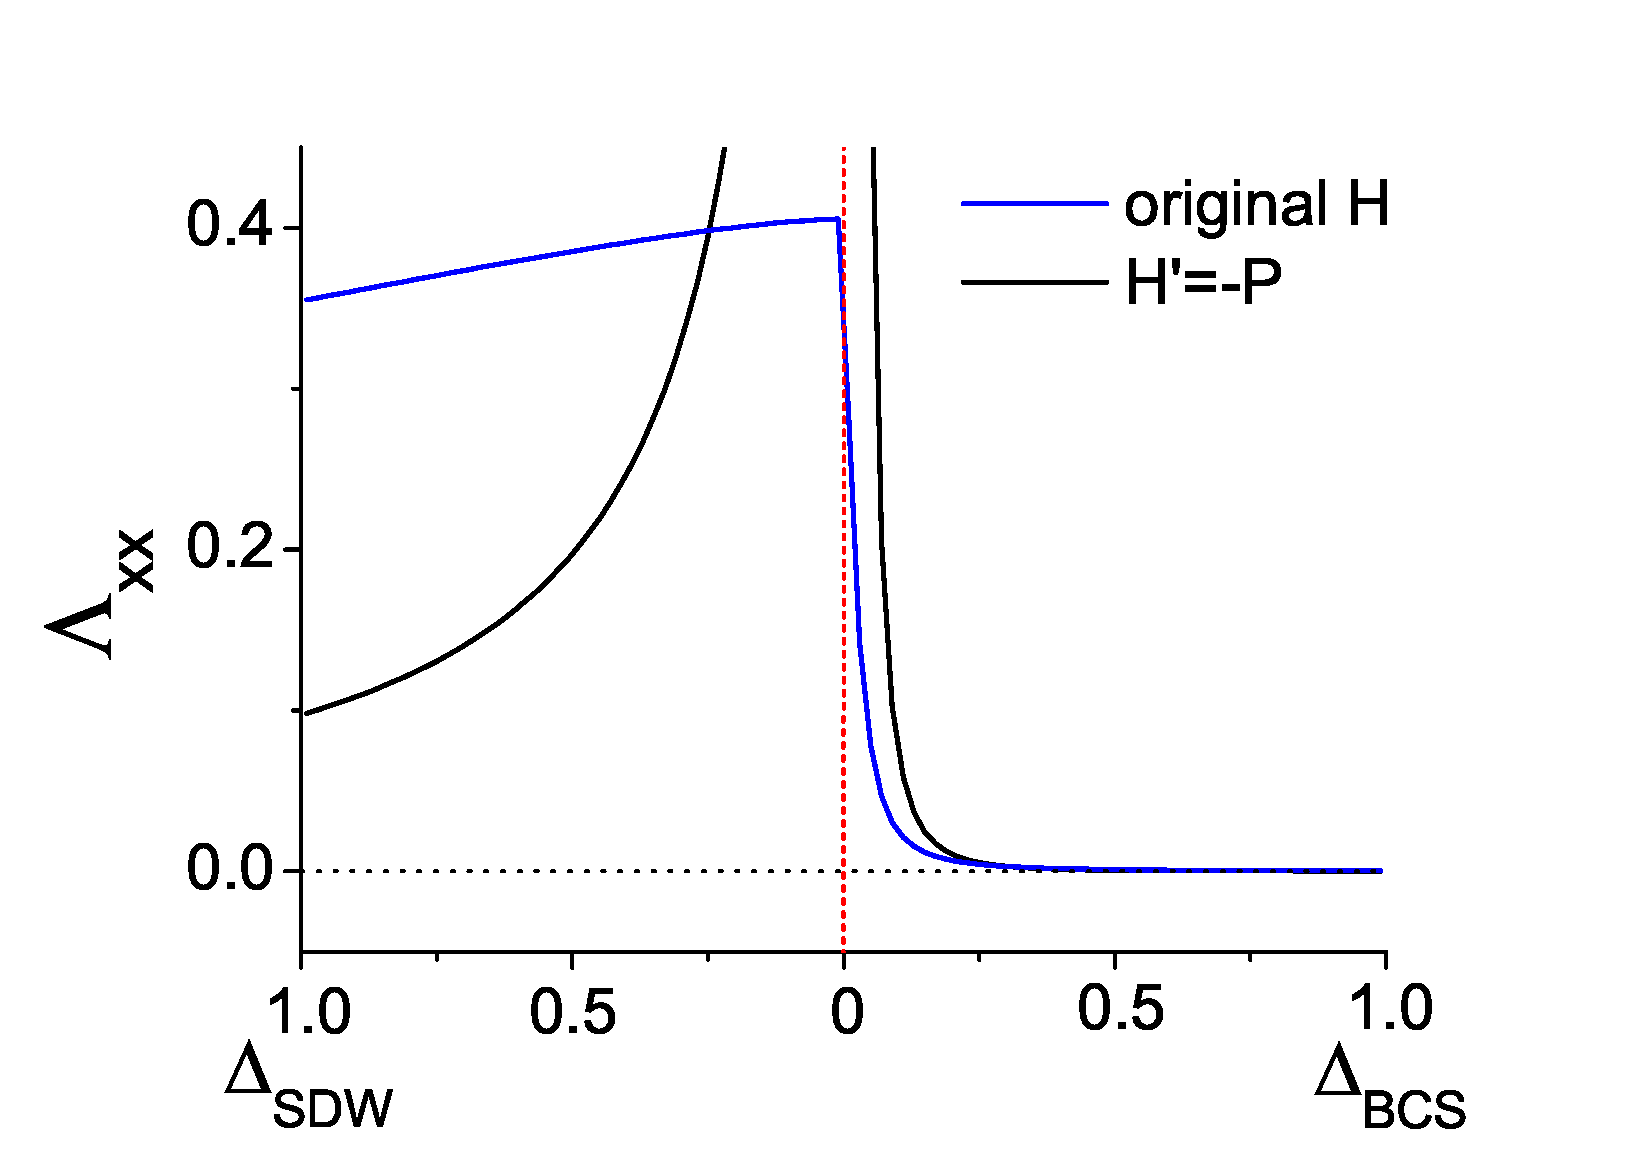
\includegraphics[scale=0.35]{figkLambda.eps}
%\caption{Static paramagnetic current-current correlation function $\Lambda_{xx}(q_x=0, q_y\rightarrow 0)$ as in Eq. \ref{eq:lambdaform} for the original mean-field Hubbard model at half filling on two-dimensional square lattice in Eq. \ref{eq:mfham} and the phase-equivalent effective model $H'=-P$. The vertical red dashed line where $\Delta_{BCS}=\Delta_{SDW}=0$ is the mean-field phase boundary between the SDW insulator and the superconductor. In comparison with the original Hamiltonian, $H'$ does induce significant quantitative changes to $\Lambda_{xx}$; however, the phase-defining qualitative feature remains intact: $\Lambda_{xx}$ vanishes rapidly in a superconducting phase consistent with the onset of the Meissner effect.}\label{fig:exact}
%\end{figure}

%We consider instead an alternative model described by $H'=-P$,  where $P = \underset{n}{\sum} |n\rangle\langle n|$ is the projection operator onto the ground state. $H'$ shares with $H$ the same group of occupied (unoccupied) states $\left|n\right\rangle$ ($\left|m\right\rangle$) yet with a flattened quasiparticle spectrum $E'_n=-1$ ($E'_m=0$). Since we expect $H'$ to be superconducting if and only if $H$ is superconducting and the two models are adiabatically connected without closing the spectrum gap, we can based our judging criteria of the Meissner effect upon $\Lambda'_{xx}$ instead of $\Lambda_{xx}$, see Fig. \ref{fig:exact}. 

%\begin{eqnarray}
%\Lambda'_{xx}&=&-\underset{q_y\rightarrow 0}{\lim} \mbox{tr} \left[P \left\{Q,\left[H', x\right]\right\} \exp(-iq_y y)(1-P) \left\{Q,\left[H', x\right]\right\}\exp(iq_y y)\right] 
%\end{eqnarray}

%\begin{eqnarray}
%\Lambda'_{xx} &=& \underset{q_y\rightarrow 0}{\lim}\mbox{tr} \left[ P  j_x(-q_y)  \left(1-P\right) j_x(q_y)\right] \\
%&=& \underset{ijkl}{\sum} L_{ijkl}\times %\left(x_i-x_j\right)\left(x_k-x_l\right)\underset{q_y\rightarrow 0}{\lim}\exp\left[iq_y(y_l-y_j)\right] \nonumber\\
%&-&\underset{jkl}{\sum} L'_{jkl}\times \left(x_j-x_k\right)\left(x_k-x_l\right)\underset{q_y\rightarrow 0}{\lim}\exp\left[iq_y(y_l-y_k)\right]\nonumber
%\end{eqnarray}

\end{document}
